%%%%%%%%%%%%%%%%%%%%%%%%%%%%%%%%%%%%%%%%%%%%%%%
%%%%%%%%%%%%%%%%%%%%%%%%%%%%%%%%%%%%%%%%%%%%%%%
%%%%%%%%%%%%%%%%%%%%%%%%%%%%%%%%%%%%%%%%%%%%%%%
%%%%%%%%%%%%%%%%%%%%%%%%%%%%%%%%%%%%%%%%%%%%%%%


この章では、宇宙の磁場研究に関する現状の科学的課題(\S \ref{c06.s1})、国際SKAの科学的課題(\S \ref{c06.s2})、日本が狙う科学的課題(\S \ref{c06.s3})をまとめる。

%%%%%%%%%%%%%%%%%%%%%%%%%%%%%%%%%%%%%%%%%%%%%%%
%%%%%%%%%%%%%%%%%%%%%%%%%%%%%%%%%%%%%%%%%%%%%%%
%%%%%%%%%%%%%%%%%%%%%%%%%%%%%%%%%%%%%%%%%%%%%%%
\setcounter{section}{0}\section{現状の科学的課題}
\label{c06.s1}

\paragraph{はじめに}

磁場は自然界の4つの基本力の1つを担う。磁場は宇宙の様々な天体に普遍的に存在し、それらのダイナミクスや高エネルギー現象の多様性を形作っている。ゆえに磁場は宇宙進化の理解に欠かせない物理量である。センチ波・メートル波の観測は、人類が磁場を探ることのできる数少ない方法の中で、大変有望な方法である。その理由として、視線に垂直な磁場成分の情報を与えるシンクロトロン放射と、視線に平行な磁場成分の情報を与える偏波ファラデー回転が、共に観測できる有利性が挙げられる。SKAはこれらを広く・深く・細かく・そして広帯域に観測することで、かつてないほど精密に磁場を計測し、宇宙磁場の理解に他に代えがたい貢献をするだろう。この節ではまずSKA宇宙磁場研究における重要な物理量や用語をまとめる。次に宇宙磁場に関する現状の科学的課題を研究領域ごとにまとめる。

%%%%%%%%%%%%%%%%%%%%%%%%%%%%%%%%%%%%%%%%%%%%%%%
%%%%%%%%%%%%%%%%%%%%%%%%%%%%%%%%%%%%%%%%%%%%%%%
\subsection{磁場研究の物理量}
\label{c06.s1.ss1}

この小節では電波観測量と磁場との基本的な関係をまとめる。特に偏波解消とファラデートモグラフィーは日本の戦略に位置づけているので本小節で詳しく紹介する。知識のある読者は次の小節に進んで頂いて構わない。式の詳しい導出については教科書\citep{1979rpa..book.....R,1996tra..book.....R}を参照されたい。

%%%%%%%%%%%%%%%%%%%%%%%%%%%%%%%%%%%%%%%%%%%%%%%
\subsubsection{シンクロトロン放射}
\label{c06.s1.ss1.sss1}

\paragraph{放射の式}

シンクロトロン放射は磁力線の周りを旋回する高速荷電粒子からの制動放射である。そして一般に我々が観測するのは宇宙線電子の集団からの放射である。そこで宇宙線電子の集団が等方的に分布すると仮定し、そのエネルギー分布を$N(\gamma)d\gamma=C(r)\gamma^{-p}d\gamma$のような冪則に従うと仮定する。ここで$\gamma$はローレンツ因子、$C(r)$は位置$r$での宇宙線電子の個数密度、$p$はスペクトル指数である。この集団が磁場$B$の中にある場合のシンクロトロン放射は、特性ストークスパラメータを$I$、$Q$、$U$、特性直線偏波強度を$P$とすると次のように書ける。
\begin{equation}
I = \int 2j(p)G_1(p)\omega^{(1-p)/2}B_\perp(r)^{(1+p)/2}C(r) dr
\end{equation}
\begin{equation}
P = Q + iU = \int 2j(p)G_2(p)\omega^{(1-p)/2}B_\perp(r)^{(1+p)/2}C(r)e^{2i\chi(r)} dr
\end{equation}
ここで単位はerg/s/cm$^2$/Hz/srであり、電波観測でよく使われるJyを用いると、10$^{23}$Jy/srである。$B_\perp$は視線に垂直な磁場の強度、$\chi$は位置$r$での初期偏波角、$\omega = 2 \pi \nu$は角振動数、$\nu$は周波数、そして$j$や$G$は係数
\footnote{
光速$c$、素電荷量$q$、電子質量$m$、$\Gamma$関数に対して
$j(p)=\frac{1}{4\pi}\frac{\sqrt{3}q^3}{8\pi mc^2}\left(\frac{2mc}{3q}\right)^{(1-p)/2}$、\\
$G_1(p)=\frac{1}{1+p}2^{(1+p)/2}
\Gamma \left(\frac{p}{4}-\frac{1}{12}\right)
\Gamma \left(\frac{p}{4}+\frac{19}{12}\right)
$、
$
G_2(p)=2^{(p-3)/2}
\Gamma \left(\frac{p}{4}-\frac{1}{12}\right)
\Gamma \left(\frac{p}{4}+\frac{7}{12}\right)
$である。
}
である。後述するファラデー回転は考えていない。式が示す通り、シンクロトロン放射強度は宇宙線電子の個数密度に比例し、磁場と周波数の冪乗に比例する。$I$、$Q$、$U$と宇宙線電子分布が分かれば、磁場の視線垂直成分の積分量が分かる。

\paragraph{強度の周波数依存性}

ここで電波強度と偏波強度の放射スペクトル指数を定義する。
\begin{equation}
I(\nu)\propto \nu^{\alpha_I},~~~P(\nu)\propto \nu^{\alpha_P}
\end{equation}
後述する偏波解消がなければ$\alpha_I=\alpha_P$であるが、偏波解消があると等号は成り立たなくなる。一般に冪は負の値をとるため、長波長ほど明るい。図\ref{c06.s1.ss1.f1}左には天の川銀河の典型的な電波放射スペクトルを示す。センチ波・メートル波ではシンクロトロン放射が自由電子の熱制動放射や回転ダスト放射に比べて支配的なのが分かる。

\paragraph{偏波率}

偏波率$\Pi$は電波強度$I$と偏波強度の比で
\begin{equation}
\Pi=(Q^2 + U^2 + V^2)^{1/2}/I
\end{equation}
と書ける。ここでストークスVは円偏波強度である。円偏波強度は太陽や恒星、ジェットなどを除き、一般に極めて小さい。そこで実務的には直線偏波だけを考えた直線偏波率
\begin{equation}
\Pi_l=|P|/I=(Q^2 + U^2)^{1/2}/I
\end{equation}
が偏波率として参照されることがある。宇宙線電子が等方的でかつ偏波解消がなければ、$\Pi_l=G_2(p)/G_1(p)$であり、$p=3$ならば0.75の値を取る(偏波率75 \%)。

\paragraph{偏波角}

偏波がなしている角度を表す偏波角$\chi$は次のように書ける。
\begin{equation}
\chi=\frac{1}{2}\arctan\left(\frac{U}{Q}\right)
\end{equation}
この偏波角はストークスパラメータを定めるポアンカレ球の定義に由来し$-\pi/4 \le \chi \le \pi/4$の範囲をとる。一方で、慣例的には$-\pi/2 \le \psi \le \pi/2$の範囲を取る電場ベクトル偏波角$\psi=2\chi$を参照することが多い。なお偏波角のゼロ点の取り方と正値をとる向きには任意性がある。伝統的な電波天文学の定義では北銀極方向をゼロとし東方向への回転を正に取る。

\begin{figure}[tbp]
\begin{center}
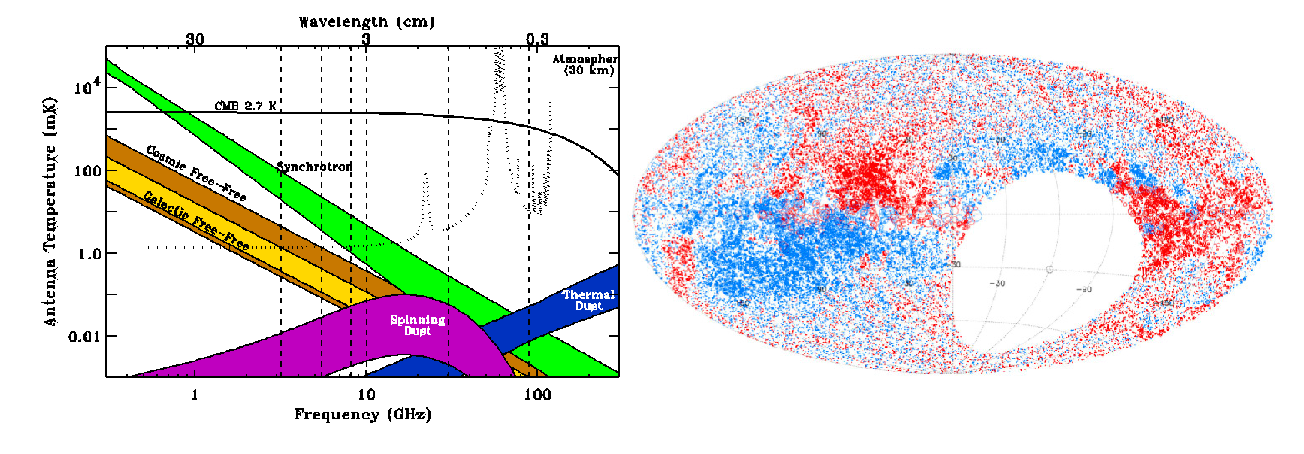
\includegraphics[width=\linewidth]{magnetism/c06.s1.ss1.f1.eps}
\caption{(左) 天の川銀河の典型的な放射スペクトル。NASAのホームページから引用。(右) 全天の系外偏波源のRMの分布\citep{2009ApJ...702.1230T}。円がそれぞれの観測点で、その大きさがRMの大きさ、赤と青は正値と負値を表す。VLAが観測できない領域が白抜きになっている。座標は銀経・銀緯。銀河中心方向(銀経0)や円盤面(銀緯0)を挟んでのRMの符号の反転が見受けられ、この大局的な構造は天の川銀河の磁場起源と理解されている。
}\label{c06.s1.ss1.f1}
\end{center}
\end{figure}

%%%%%%%%%%%%%%%%%%%%%%%%%%%%%%%%%%%%%%%%%%%%%%%
\subsubsection{直線偏波ファラデー回転}
\label{c06.s1.ss1.sss2}

\paragraph{回転測度RM}

直線偏波ファラデー回転は偏波が磁気流体中を通過する際に偏波角が回転する現象である。通過前の偏波角を$\chi_0$とすると、通過した後の偏波角$\chi$は波長$\lambda$の2乗に比例し、
\begin{equation}
\chi=\chi_0+RM\lambda^2
\end{equation}
と書ける。ここで係数$RM$をファラデー回転測度と呼ぶ。この関係から、2つ以上の異なる波長で偏波角を測定すると、その回転角度差がRMを与える。式にすると
\begin{equation}
RM =\frac{\chi(\lambda_1)-\chi(\lambda_2)}{\lambda_1^2-\lambda_2^2}
\end{equation}
となる。添字の1と2は異なる波長を意味する。ファラデー回転測度は物理的には
\begin{equation}
RM~({\rm rad~m^{-2}}) \approx 0.8119 \int 
\left(\frac{n_{\rm e}}{\rm cm^{-2}}\right)
\left(\frac{B_{||}}{\rm \mu G}\right)
\left(\frac{dr}{\rm pc}\right)
\end{equation}
と書ける。$n_{\rm e}$は自由電子密度、$B_{||}$は磁場の視線に平行な成分、$r$は視線距離である。積分は観測者に向けてなされ、磁場が観測者を向いている場合RMが正値である。偏波$Q$、$U$から$\chi$を求め(式6.6)、$\chi$の波長依存からRMを求め(式6.7, 6.8)、そして自由電子分布を何らかの方法で与えれば、磁場の視線平行成分の積分量が式6.9から分かる。さらにファラデー回転を逆算すれば、放射位置での偏波角が式6.7から分かり、通常のシンクロトロン放射であればそれに直交する向きが視線に垂直な磁場の向きである。ただし向きが南北方向と分かったとしても、北から南か、南から北か、どちらを向いているのかまでは分からない。

\paragraph{RMの全天カタログ}

RMの測定はその電離物質自身が放射している必要がなく、背景に偏波源があればよい。幸い、宇宙のほとんどの天体はシンクロトロン偏波を放っている。例えば系内ではパルサー、系外ではクェーサーや電波銀河が、銀河や銀河団のRM観測に役立っている。図\ref{c06.s1.ss1.f1}右はVLAのNVSS全天サーベイで得られた37543個の銀河系外天体のRMを示す\citep{2009ApJ...702.1230T}。これが執筆時最大のRMカタログである。

\paragraph{RMの観測可能範囲}

ファラデー回転は短波長ほどRMに対する回転角度が小さい。ゆえに偏波角の測定精度に波長によらない誤差があると、短波長ほどRMの決定精度は悪くなる。つまり小さなRMは短波長では観測しずらい。一方で長波長ほど同じRMに対して偏波角が半回転以上してしまう$n\pi$不定性を伴いやすい。つまり大きなRMは長波長では観測値に不定性がある。SKAが網羅するセンチ波・メートル波は、ミリ波・サブミリ波やデカメートル波では難しい、多くの天体の標準的な${\rm RM} \sim O(1-1000)$~rad m$^{-2}$を観測できる唯一無二の帯域なのである。

%%%%%%%%%%%%%%%%%%%%%%%%%%%%%%%%%%%%%%%%%%%%%%%
\subsubsection{偏波解消}
\label{c06.s1.ss1.sss3}

\paragraph{原理}

偏波解消(depolarization)とは、放射された偏波よりも弱まった偏波強度を観測する現象のことである。偏波解消は、放射物質の特性、放射が伝搬する空間物質の特性、そして観測の特性に依存する。以下にいくつかの偏波解消の事例を挙げる。
\begin{itemize}
\item 波長非依存偏波解消(Wavelength independent depolarization)\\
シンクロトロン偏波を起こしている磁場が非一様である場合に起こる。観測するビームの中で偏波が視線ごとに異なる偏波角を持って放射され観測者に届くために、ビーム内で偏波の打ち消し合いが起こりうる。
\item 差分ファラデー回転偏波解消(Differential Faraday rotation depolarization)\\
シンクロトロン偏波を放つ宇宙線電子とファラデー回転を引き起こす熱的電子が混在する場合に起こる。視線上で奥側の偏波と手前側の偏波が同じ偏波角で放射されたとしても、2つが異なるファラデー回転をして観測者に届くために、偏波の打ち消し合いが起こりうる。
\item ビーム偏波解消(Beam depolarization)\\
観測するビームの中でRMに構造がある場合に起こる。ビーム内の偏波が仮に同じ偏波角で放射されたとしても、ビーム内の視線ごとに異なるファラデー回転をして観測者に届くために、偏波の打ち消し合いが起こりうる。
\item バンド幅偏波解消(Bandwidth depolarization)\\
観測する周波数帯域幅が広い場合に起こる。基本的に放射時の偏波角は波長によらないが、波長によって異なるファラデー回転をして観測者に届くために、周波数積分をした場合に偏波の打ち消し合いが起こりうる。
\end{itemize}

\paragraph{Burnの法則}

\cite{1966MNRAS.133...67B}はいくつかの単純な状況下での偏波解消の定式化を試みた。それらは広くBurnの法則として知られている。まず差分ファラデー回転偏波解消の解析解を紹介する。シンクロトロン放射とファラデー回転を起こす領域があり、それが完全に一様な磁場を持つ場合、観測される直線偏波率は以下の正弦関数で書ける。
\begin{equation}
\Pi_l(\lambda^2) = \Pi_{l0}(\lambda^2)
\frac{\sin \left( RM \lambda^2 \right) }{RM \lambda^2}
\exp{2i \left(  \chi_0 + \frac{1}{2}RM \lambda^2 \right) }.
\end{equation}
ここで、$\Pi_l, \Pi_{l0}$はそれぞれ観測される直線偏波率と本来の直線偏波率である。このような法則に従う領域をBurn slabと呼ぶこともある。次にビーム偏波解消の解析解を紹介する。乱流磁場が存在しているような状況で、ビーム内のRMの分布が正規分布に従い、その分散が$\sigma_{\rm RM}$と定量化できる場合に、観測される直線偏波率は以下の指数関数で書ける。宇宙線電子と混在している場合(内部ファラデー分散型の偏波解消、internal Faraday dispersion depolarization)は
\begin{equation}
\Pi_l(\lambda^2) = \Pi_{l0}(\lambda^2)
\frac{1-\exp \left(-2\sigma_{\rm RM}^2 \lambda^4\right)}{2\sigma_{\rm RM}^2 \lambda^4}
\end{equation}
と書け、放射領域の前景として存在している場合(外部ファラデー分散型の偏波解消、external Faraday dispersion depolarization)は
\begin{equation}
\Pi_l(\lambda^2) = \Pi_{l0}(\lambda^2)\exp \left(-2\sigma_{\rm RM}^2 \lambda^4\right)
\end{equation}
と書ける。図\ref{c06.s1.ss1.f2}にはBurnの法則を示したものをまとめる\citep{2011MNRAS.418.2336A}。

\begin{figure}[tbp]
\begin{center}
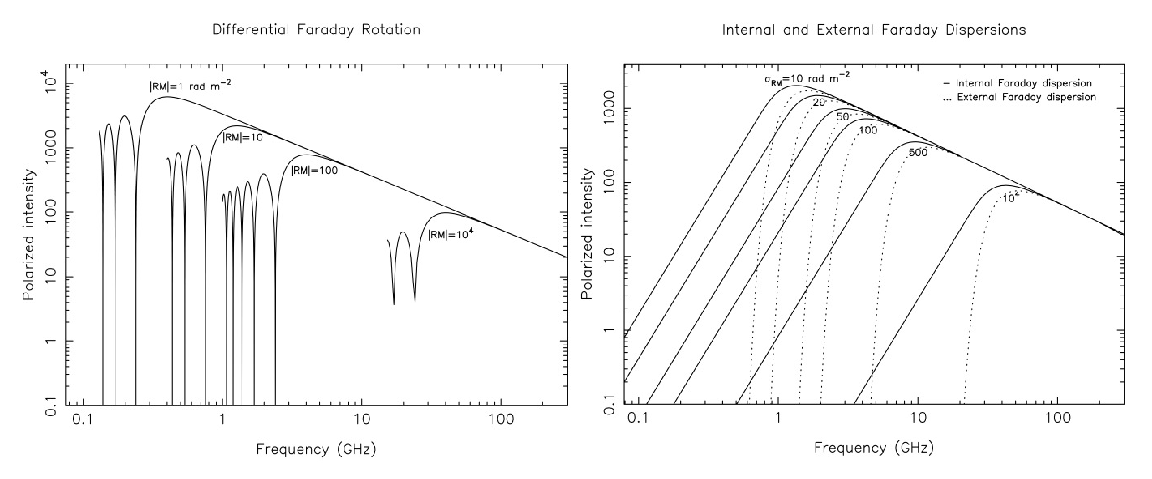
\includegraphics[width=1.0\linewidth]{magnetism/c06.s1.ss1.f2.eps}
\caption{左図は差分ファラデー回転偏波解消、右図は内部・外部ファラデー分散偏波解消の様子。RMの大きさによってスペクトルの折れ曲がる周波数が異なる。\citep{2011MNRAS.418.2336A}。
}\label{c06.s1.ss1.f2}
\end{center}
\end{figure}

\paragraph{偏波解消の回避}

Burnの法則を用いれば、観測した偏波解消からRMやRMの分散が推定できる。その際より精度よく調べるには、偏波解消の影響を受けていないデータもあると良い。例えば、差分ファラデー回転偏波解消やバンド幅偏波解消は短波長ほど起こりにくい。多くの天体の標準的なRM $O(1-1000)$~rad m$^{-2}$に対しては、SKAの範囲内(数-10GHz帯)で観測することで偏波解消は克服できる。ビーム偏波解消や波長非依存偏波解消は、高い空間分解能による観測で回避することができる。SKAは従来(たとえばJVLA)よりも一桁近く向上した$1''$を下回る空間分解能を有することができるので、従来より偏波解消を克服した観測が実現できるだろう。

%%%%%%%%%%%%%%%%%%%%%%%%%%%%%%%%%%%%%%%%%%%%%%%
\subsubsection{ファラデートモグラフィー}
\label{c06.s1.ss1.sss4}

\paragraph{原理}

直線偏波磁場断層解析法(ファラデートモグラフィー)は視線上の物質構造を推定する新しい手法として世界的に注目されている。RMは視線積分量を与えるが、ファラデートモグラフィーは視線分布を与える。その原理についてここで簡単にまとめる。特性直線偏波強度Pの式に立ち戻ると、ファラデー回転まで考えて、それは次のように書ける。
\begin{equation}
P(\lambda^2)=\int \varepsilon(r)e^{2i\chi(r,\lambda^2)}dr
\end{equation}
ここで積分は視線方向$r$について、$\varepsilon(r)$は位置$r$での放射率、
\begin{equation}
\chi(r,\lambda^2)=\chi_0(r)+\phi(r)\lambda^2
\end{equation}
は観測者の位置での偏波角、$\chi_0(r)$は放射した位置$r$での初期偏波角である。$\phi(r)$はRMと同じ物理量だが、位置$r$までのRMということを明確にするために、ファラデー深度と呼ばれる。さて、積分変数を$r$から$\phi(r)$へ変換すると、$\phi$は$\infty$から$-\infty$までの値を取り得るので、
\begin{equation}
P(\lambda^2)=\int^\infty_{-\infty}F(\phi)e^{2i\phi\lambda^2}d\phi
\end{equation}
\begin{equation}
F(\phi) \equiv \varepsilon(\phi)e^{2i\chi_0(\phi)}
\end{equation}
と書けるのが分かるだろうか。この$F(\phi)$はファラデー分散関数、またはファラデースペクトルと呼ばれ、$\phi$空間での偏波強度分布を表している。さて、変換された式を見ると、$\phi$と$\lambda^2$を共役変数とするフーリエ変換の形になっていることが分かる。ゆえに逆変換
\begin{equation}
F(\phi)=\frac{1}{2\pi}\int^\infty_{-\infty}P(\lambda^2)e^{-2i\phi\lambda^2}d\lambda^2
\end{equation}
が存在し、つまり、観測量$P(\lambda^2)$から$F(\phi)$を推定できる。もしファラデー深度の分布が物理距離に対して単調であれば、これは偏波強度とRMを視線方向に断層解析したことに他ならない。これが\citet{1966MNRAS.133...67B}によって提唱されたファラデートモグラフィーの原理である。

\paragraph{ファラデートモグラフィーの実用}

逆変換によるファラデースペクトルの推定は、しかしながら、現実には$\lambda^2$空間の全ての点を観測することが不可能であるため不完全である。観測可能波長の偏波強度だけで再構築されるファラデースペクトル$\tilde F(\phi)$は、窓関数$W(\lambda^2)$を用いて
\begin{equation}
\tilde F(\phi)=\frac{1}{2\pi}\int_{-\infty}^\infty W(\lambda^2)P(\lambda^2)e^{-2i\phi\lambda^2}d\lambda^2
\end{equation}
のように書ける。この式はさらに畳込みの定理を用いて、
\begin{equation}
\tilde F(\phi)=K^{-1}R(\phi)\ast F(\phi)
\end{equation}
\begin{equation}
R(\phi)=K\int^\infty_{-\infty} W(\lambda^2)e^{-2i\phi\lambda^2}d\lambda^2
\end{equation}
\begin{equation}
K=\left[\int^\infty_{-\infty} W(\lambda^2)d\lambda^2\right]^{-1}
\end{equation}
と書ける。これはつまり、再構築されるファラデースペクトルの品質は$R(\phi)$の品質で定まっていることを示している。この$R(\phi)$は回転測度波及関数(RMSF)と呼ばれる。$R(\phi)/K$がデルタ関数$\delta(\phi)$であれば完全な再構築になるが、現実には起こりえない。図\ref{c06.s1.ss1.f3}にはRMSFの例を示す。

\paragraph{ファラデートモグラフィーの分解能と範囲}

RMSFの半値幅(FWHM)がファラデートモグラフィーのRM分解能の目安である。例として窓関数が観測可能な波長帯($\lambda^2_{\rm min} \leq \lambda^2\leq \lambda^2_{\rm max}$)で$W(\lambda^2)=1$、その他で0の値をとる場合、RMSFのFWHMは
\begin{equation}
{\rm FWHM~(rad~m^{-2})} = \frac{2\sqrt3}{\Delta\lambda^2({\rm m^2})},
\quad \Delta\lambda^2 = \lambda^2_{\rm max} - \lambda^2_{\rm min}
\end{equation}
と書け、波長2乗空間の範囲がRM分解能を決めていることが分かる。特に長波長側の観測帯域を増やすと、効果的に積分範囲が拡大しRM分解能が向上する。一方で、長波長にいくと偏波解消が無視できなくなる。偏波解消が強く起こる目安は偏波角が$\pi$だけ回転するRMと波長の関係に他ならないので、観測可能な最大のRM構造は次のように書ける。
\begin{equation}
L_{\rm \phi, max}~{\rm~(rad~m^{-2})} \approx \frac{\pi}{\lambda^2_{\rm min}({\rm m^2})}
\end{equation}
効果的にトモグラフィーをするにはこれら2つの制限を同時に改善する必要がある。それがSKAなどの広帯域観測の実現によってトモグラフィーが急速に実用化されつつある理由である。

\begin{figure}[tbp]
\begin{center}
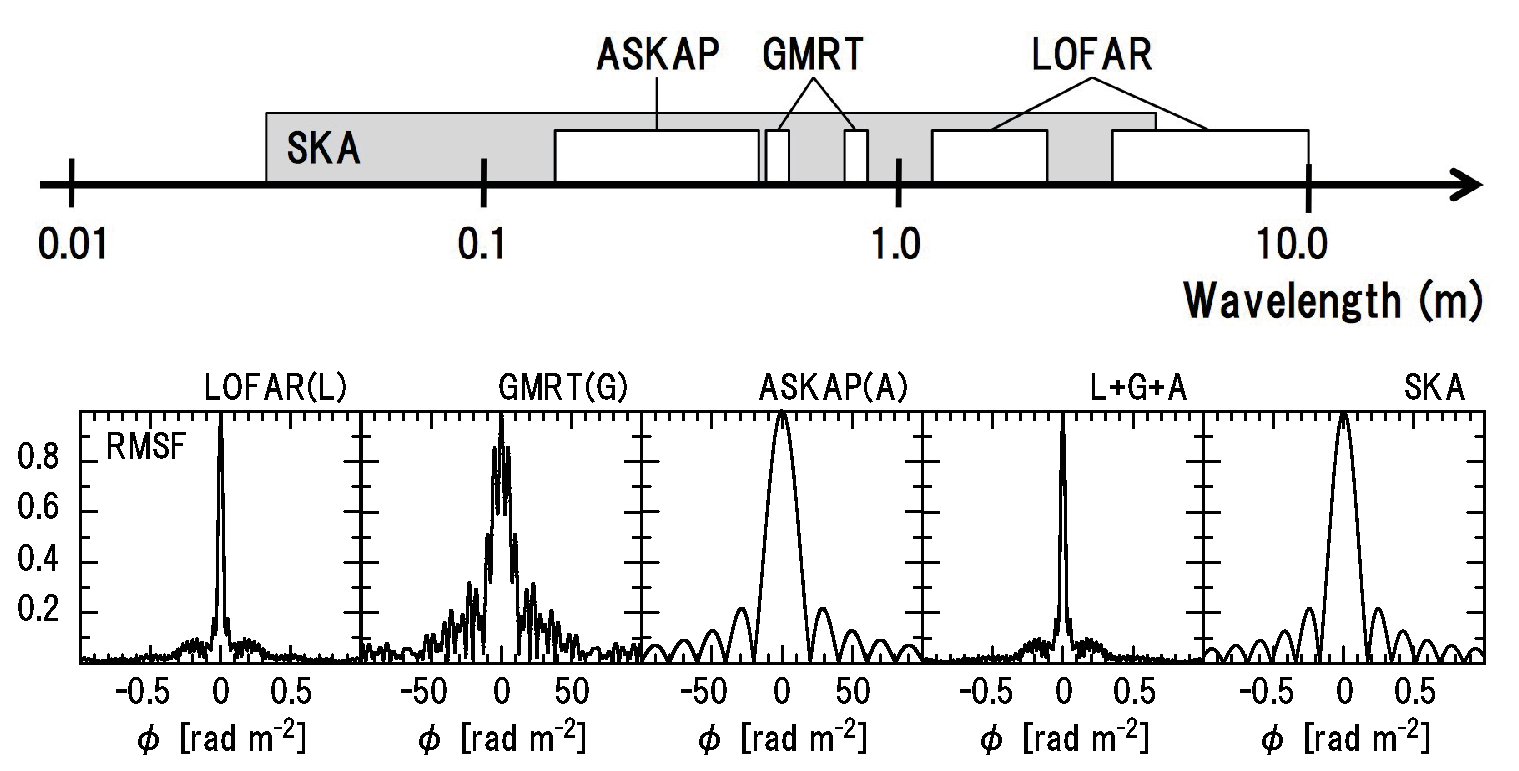
\includegraphics[width=0.7\linewidth]{magnetism/c06.s1.ss1.f3.eps}
\caption{回転測度波及関数(RMSF) $R(\phi)$の例\citep{2014PASJ...66...65A}。横軸のスケールが異なることに注意。SKA以上に長波長まで網羅するLOFARの方がRMSFのメインピークの幅がSKAより狭く、すなはちファラデースペクトルの分解能は高い。しかし数10 ${\rm rad~m^{-2}}$以上に広がったファラデースペクトルに感度がない。多くの天体の標準的なRM $O(1-1000)$~rad m$^{-2}$を探るには、SKAの帯域でシームレスに観測するのがもっとも良い。
}\label{c06.s1.ss1.f3}
\end{center}
\end{figure}


%%%%%%%%%%%%%%%%%%%%%%%%%%%%%%%%%%%%%%%%%%%%%%%
%%%%%%%%%%%%%%%%%%%%%%%%%%%%%%%%%%%%%%%%%%%%%%%
\subsection{星間・天の川銀河磁場の科学的課題}
\label{c06.s1.ss2}

%%%%%%%%%%%%%%%%%%%%%%%%%%%%%%%%%%%%%%%%%%%%%%%
\subsubsection{はじめに}
\label{c06.s1.ss2.sss1}

\paragraph{天の川銀河と星間ガス}

天の川銀河は約2兆個の恒星の集団である。恒星の大部分は半径約15-20~kpc程度の円盤状に分布し、円盤内に渦巻き状に明るく輝く渦状腕を形成しながら、天の川銀河中心に対して公転運動をしている。太陽は銀河中心から約8 kpc離れた円盤部に位置する。また恒星は円盤部を大きく取り囲むハローと呼ばれる空間にも広く分布している。恒星と恒星との間の星間空間には水素が主成分の星間ガスが存在し、星間ガスの総質量は恒星の総質量の10分の1程度、円盤部での平均数密度は約$1$ cm$^{-3}$である。ガスは主に温度の違いを反映して、水素分子で構成された分子雲、水素原子で構成されたHIガス、そして電離水素のHIIガスと呼ばれ分類されている。分子雲は低温高密度の状態にあり恒星を生み出している。HIガスは円盤部において質量や体積の大部分を占めている。それぞれのガスの温度や密度は異なるが、圧力はほぼ同じ値に保たれている。さらに、ハローにはX線で観測されるような高温ガスも存在する。

\paragraph{星間ガスが帯びる磁場}

星間ガスには一般に星間磁場が付随する。天の川銀河には平均的には渦状腕に沿うような大局的に整列した磁場が存在し\citep{1986ARA&A..24..459S}、その強さは3 $\mu$G 程度である。これと同時に局所的にはランダムな磁場成分も存在し、その強さは5 $\mu$G 程度である\citep{1406.0283}。ランダムな磁場は主に星間ガスの乱流に起因しており、コルモゴロフ則の乱流のエネルギースペクトルが確認されている。その乱流磁場の相関長は渦状腕で20 pc、渦状腕の間で100 pc程度と見積もられている\citep{2006ApJ...637L..33H}。ハローにおいても円盤部と同程度のおよそ10 $\mu$G以下の大局・局所磁場が存在することが示唆されている\citep{1406.0283}。天の川銀河ではさらに、銀河中心に強い磁場($\sim 50$ $\mu$G)が観測されている\citep{2010Natur.463...65C}。

\paragraph{星間磁場と宇宙線の関係}

宇宙線は高エネルギーの粒子で、その大部分は超新星爆発などによって加速された陽子と考えられている。単位体積あたり、宇宙線のエネルギーは星間ガスの内部エネルギーや磁場のエネルギーとおおよそ同程度である\citep{2001RvMP...73.1031F}。荷電粒子の宇宙線は磁場から力を受けて運動する。そして宇宙線の運動は磁場を介して星間ガスに圧力として影響を及ぼす。ゆえに、星間ガスの力学には磁場と同様に宇宙線の圧力も無視できない\citep{1966ApJ...145..811P}。

%%%%%%%%%%%%%%%%%%%%%%%%%%%%%%%%%%%%%%%%%%%%%%%
\subsubsection{星間磁場の理論}
\label{c06.s1.ss2.sss2}

\paragraph{磁場の起源と2つの不安定性}

銀河の磁場を説明するひとつのモデルとして、ダイナモモデルが提唱されている\citep{1971ApJ...163..255P}。これは銀河の回転の運動エネルギーや乱流の運動エネルギーを磁場のエネルギーに変換するモデルである。また、近年、以下に述べる磁気回転不安定性も星間磁場の増幅機構として注目されている。ここでは、大スケールの星間ガスにおいて重要と考えられる二つの不安定性について紹介する。

\paragraph{磁気回転不安定性}

磁気回転不安定とは、差動回転する円盤のプラズマガスにおいて、ガスを貫く磁場により角運動量が内側から外側に輸送されて生じる。内側のガスは角運動量を失って落下し、外側のガスは角運動量を得て外向きに移動する。この際磁力線が伸張され、磁場を効率的に増幅する。しかし小スケールの磁場を生成しやすく、銀河の大局的に整列した磁場を形成できるのかは未解明である。事実、磁気回転不安定性で成長した小スケールの磁場は様々な方向を向いているので、円盤内で相殺してしまう。つまり、磁気回転不安定性は磁気エネルギーを増幅できるが、大局磁場となる磁束を増幅できない。円盤内で大局的に磁場が増幅するためには、磁気回転不安定性が成長するのみではなく、円盤から磁束の一部が逃げていく効果が必要であることが、銀河ガス円盤の数値実験から示されている\citep{2006ApJ...641..862N}。

\paragraph{パーカー不安定性}

パーカー不安定とは、重力場中のプラズマガスが磁気圧によって持ち上げられている時の重力エネルギーを開放することによって生じる。ガスが磁気ループに沿って落下すると同時に、磁気ループは浮力を得て上空へと膨張する。前述において円盤から磁束が逃げていく物理機構がパーカー不安定である。つまり大局的な磁場の増幅においては磁気回転不安定性だけでなくパーカー型の浮力効果(従って密度の成層構造)も重要である。ここで、銀河の星間ガスを考える時、パーカー不安定性に大きな影響を与える要素が宇宙線である。宇宙線の影響については日本のサイエンス(\S \ref{c06.s3.ss2})にて詳しく紹介する。

%%%%%%%%%%%%%%%%%%%%%%%%%%%%%%%%%%%%%%%%%%%%%%%
\subsubsection{星間磁場の観測}
\label{c06.s1.ss2.sss3}

\paragraph{パルサー観測}

天の川銀河の星間磁場を測定する有力な手段の一つは、パルサーのパルス分散とファラデー回転を共に観測することである。ここでパルス分散とは、電波がプラズマ中を伝搬する際その伝搬速度が波長により異なるため、パルスを観測するとパルス到達時刻が波長で分散する現象である。電離ガスの数密度を$n_e$、パルサーまでの距離を$L$とすると、パルスが通過した電離ガスの密度と距離との積(分散測度, DM)は${\rm DM} = \int n_e dr$と書く事ができる。これとRMの式(式6.9)との比をとると、磁場の視線方向の強さの密度重み付き平均値を見積もることができる。今のところ、パルサーの数が少なく($\sim 10^3$個程度)、またパルサーまでの距離が曖昧なため、天の川銀河のどの位置の星間磁場を測定しているのかという点に不確かさが残っているが、SKAでパルサーアストロメトリが進めば、大きく改善されると期待されている。

\paragraph{背景の系外偏波源観測}

パルサーの代わりに遠方の銀河が発した電波のRMを参照することもできる。図\ref{c06.s1.ss1.f1}右にはVLAのNVSS全天サーベイで得られた37543個の系外の天体のRMを示したが、このカタログの登場によって天の川銀河の磁場研究は大きく進展した。この方法ではパルサーより数が多いため、天球上においてよりきめ細いRMのマップを得ることができ、細かく磁場分布を探ることができる。デジタルカメラで言うところのピクセル数が多いのである。しかし、パルサーと異なり電離ガスの密度を直接求める方法がないため、視線方向に存在するガス密度の分布モデルを仮定しなくてはならない。また、視線方向にあるすべての磁場が積分された値で得られるため、星間磁場の局所的な情報に還元するためには、磁場分布のモデルも必要となる。

\paragraph{課題}

星間磁場の構造の全容はよく分かっていない。それは、主に私たちが天の川銀河に属している事に由来する(森の中にいると森の全体像をつかみにくいことに似ている)。全貌がはっきりしないために、その起源の理論的解明も十分に進んでいない。SKAに期待されることは、特徴的な磁場構造を見つけること、そしてその観測精度をあげることである。例えば最近、太陽より銀河中心側の銀河円盤で、大局円盤磁場の向きが反転している(例:時計回りが反時計回りに)という結果が、パルサー・系外偏波源のRMデータから分かった\citep{1406.0283}。SKAでこういった観測が進めば、そのような構造を説明する理論に議論を絞り込んでいくことが可能になる。


%%%%%%%%%%%%%%%%%%%%%%%%%%%%%%%%%%%%%%%%%%%%%%%
%%%%%%%%%%%%%%%%%%%%%%%%%%%%%%%%%%%%%%%%%%%%%%%
\subsection{系外銀河磁場の科学的課題}
\label{c06.s1.ss3}

%%%%%%%%%%%%%%%%%%%%%%%%%%%%%%%%%%%%%%%%%%%%%%%
\subsubsection{はじめに}
\label{c06.s1.ss3.sss1}

\paragraph{系外銀河と磁場}

これまでの観測から、近傍ならびに遠方の系外銀河でも磁場の存在が確認されている。ゆえに銀河の磁場は天の川銀河に限ったことではない。系外銀河では、銀河の全体を外から俯瞰できること、サンプルが1つだけではないことから、銀河磁場の多様性や時間進化、さらには星形成や銀河形態との関連など、多岐にわたる研究が可能と期待される。

%%%%%%%%%%%%%%%%%%%%%%%%%%%%%%%%%%%%%%%%%%%%%%%
\subsubsection{系外銀河磁場の理論}
\label{c06.s1.ss3.sss2}

系外銀河の磁場の理論的課題は前節の星間・天の川銀河磁場と基本的に共有している。加えて系外銀河では、早期型や晩期型といった形態、星形成の程度、銀河中心核の活動性、などと磁場との関係性にも興味が広がる。銀河磁場は星間ガスに付随するゆえに、磁場の歴史と星間ガスの歴史は不可分であり、物質循環のサイクルをなす星形成史とも不可分だろう。ファラデー回転を起こすプラズマの密度は、星間ガスが星になるにつれて減少するので、銀河のRMは緩やかな赤方偏移進化をするかもしれない。また、超新星爆発や星風のフィードバックが断続的に乱流場を駆動し、プラズマや磁場を円盤からハロー、そして銀河間空間へと輸送しうる。これらフィードバックも星形成率と関係するはずである。銀河風、ラム圧、AGN活動などを通じて、銀河磁場は銀河間物質とも結びついていると考えられる。

%%%%%%%%%%%%%%%%%%%%%%%%%%%%%%%%%%%%%%%%%%%%%%%
\subsubsection{近傍の系外銀河磁場の観測}
\label{c06.s1.ss3.sss3}

\paragraph{大局磁場}

系外銀河にも大局的な磁場が存在する。NGC6946銀河やNGC2997銀河、M83銀河では、渦状腕の間の領域で整列磁場が強い傾向がある。銀河腕の差動回転でおこる回転ずれ(シアー)の強い領域、ガス圧縮が生じる領域、乱流が小さい領域で、磁場の整列が見られる。一方で、磁場の整列度合いは星形成と相関しないことが示唆されている。天の川銀河で検出された円盤磁場の反転\citep{2011ApJ...728...97V}は、分解能が十分であるにもかかわらず見つかっていない。

\paragraph{乱流磁場}

系外銀河にも乱流磁場が存在する。偏波解消を用いてRMの分散とその空間特性が議論されており、乱流磁場の相関長は50 pcと見積もられている\citep{2007A&A...470..539B}。角度分散解析を5 GHz高分解能データに適用した研究では、 乱流磁場のうち、整列磁場に対して平行な成分の相関長は100 pc、垂直な成分の相関長は50 pcと見積もられた\citep{2013ApJ...766...49H}。1.4 GHz偏波マップの勾配解析からは、電離ガスは亜音速または臨界点にあると示唆された\citep{2012ApJ...749..145B}。

\paragraph{ハロー磁場}

系外銀河ではハローの研究も進んでいる。$\alpha$-$\Omega$ダイナモ理論によると円盤磁場はハローに弱いポロイダル磁場を伴うはずで、実際にX字型の磁場が観測的に見つかっている\citep{2014arXiv1401.1317K,2011A&A...531A.127S}。NGC253銀河のスケールハイトと宇宙線電子寿命から、アウトフロー速度が脱出速度を超える300 km/sであるという研究も電波観測で行われた\citep{2009A&A...506.1123H}。この宇宙線電子の起源は不明で、電波とガンマ線の比較を行うことによって、宇宙線電子がハドロン起源かレプトン起源かを切り分けられるだろう。

\paragraph{銀河形態と磁場}

AGNを伴わないSa型銀河、S0型銀河、楕円銀河は星形成がなく、宇宙線電子が少なく、シンクロトロン放射が見えない。しかし、渦巻銀河に類推されるように、差動回転による磁気回転不安定性やパーカー不安定性、小スケールダイナモにより、大局・局所磁場が存在する可能性がある。矮小銀河はダイナモによる増幅が起きにくいと考えられるが、IC10銀河などでは大局磁場が観測されており、銀河形成を解明する上で重要な天体である。大小マゼラン雲も回転速度が小さいにもかかわらず、ファラデー回転観測によると整列磁場が確認されている。

\paragraph{磁場とガス力学}

銀河には速い磁気音波と遅い磁気音波が存在することが、2次元MHD計算などから分かる。速い磁気音波は棒渦巻き銀河における爆発的星形成リングを形成し、遅い磁気音波はパーカー不安定を生じさせる。NGC6946銀河やM51銀河の磁場はこれらで上手く説明される。棒渦巻き銀河では、磁場形状はガスの動径運動を反映しており、銀河中心では強い磁場(50-100 $\mu$G)の影響でガスが中心部へ流入し星形成を活発化させているようである\citep{2005A&A...444..739B}。

\paragraph{電波-遠赤外線の相関}

銀河の電波連続波および遠赤外線の放射強度は良く相関する\citep{2003ApJ...586..794B}。強度スケール4桁にわたってこの相関は成立しており、kpcスケールの分解能でマッピングした観測データでも渦状腕の間も含めて成立している\citep{2011AJ....141...41D}。この相関関係は$z=3$から現在$z=0$に至るまで進化しない\citep{2008ApJ...678..828M}。光学的に厚い場合については、この熱的放射(遠赤外線)と非熱的放射(電波)の相関関係は、ダスト加熱と超新星爆発頻度が大質量星の個数密度と相関していることにより生じると解釈されている。また光学的に薄い場合では、磁場とガスの非線形な関係で相関が生じるためと解釈されている。相関のべきは領域ごとに異なり、宇宙線電子の拡散距離よりも小スケールでは相関が成立しなくなる。磁場の整列度は宇宙線電子の伝搬に関係すると考えられるため、磁場は電波-赤外線関係の理解にも重要な要素である。

\paragraph{課題}

本質的な課題は、観測サンプルが全く少ない点にある。現在までに主要なサーベイとなっているWSRT-SINGS\citep{2007A&A...461..455B,2009A&A...503..409H,2010A&A...514A..42B}でも34個の近傍銀河にとどまる。さまざまに分類分けして磁場の普遍性や多様性を探るためには、分類ごとに数10のサンプルは必要で、ゆえに数100の近傍系外銀河サンプルが最低でも求められる。上記の結果の普遍性を追求するためには、SKAで大集光力を実現し銀河サンプルを桁で増やすしかない。


%%%%%%%%%%%%%%%%%%%%%%%%%%%%%%%%%%%%%%%%%%%%%%%
\subsubsection{遠方の系外銀河磁場の観測}
\label{c06.s1.ss3.sss4}

\paragraph{観測の現状}

電波放射に関しては、感度が全く足りないため、赤方偏移$z$が$0.1$を超えるような系外銀河観測はほとんど達成されていない。ファラデー回転と偏波解消を用いた方法では、いわゆる吸収線系として振る舞う介在銀河の調査が最近進みつつある(国際サイエンス\S \ref{c06.s2.ss3}を参照)。

\paragraph{課題}

小スケールの磁場が乱流によって素早く構築される一方で\citep{2012PhRvE..85b6303S}、そろった大局的磁場は長い時間(円盤の回転周期程度)をかけて構築されると期待される\citep{2005PhR...417....1B}。\cite{2009A&A...494...21A}の数値実験によれば、もし$z=3$において銀河円盤でkpcスケールの$\mu$G強度の磁場が作られたなら、それが銀河スケールの整列した磁場に成長するには$z=0.5$程度までかかる。その間、特に星形成が盛んだった赤方偏移$z=2$から現在まで、星形成の影響も重要だろう。SKAに大集光力を与え、高遠方の銀河までも観測することで、直接観測して検証することが重要である。ファラデー回転や偏波解消に関しても、背景の探知できる偏波源を増やせば、より本格的な議論が可能になる。プラズマの密度は銀河のシンクロトロン偏波、ファラデー回転と偏波解消、そしてゼーマン効果を通じて探ることができると見込まれる。


%%%%%%%%%%%%%%%%%%%%%%%%%%%%%%%%%%%%%%%%%%%%%%%
%%%%%%%%%%%%%%%%%%%%%%%%%%%%%%%%%%%%%%%%%%%%%%%
\subsection{AGN・ジェット磁場の科学的課題}
\label{c06.s1.ss4}

%%%%%%%%%%%%%%%%%%%%%%%%%%%%%%%%%%%%%%%%%%%%%%%
\subsubsection{はじめに}
\label{c06.s1.ss4.sss1}

\paragraph{活動銀河中心核(AGN)}

銀河の中心には$10^6$ -- $10^9$太陽質量の超巨大ブラックホールが存在する。例えば天の川銀河の中心領域には${\rm Sgr A^{*}}$と名付けられたブラックホールが存在し、電波からX線まで幅広い波長で、突然増光するフレア現象や激しい時間変動などの活動性が観測されている。加えて、例えばM87銀河では、母銀河の数百倍にも及ぶジェットと呼ばれる噴出流も観測されている。このような活動性は、銀河中心巨大ブラックホールとその周りに存在する降着円盤によって引き起こされていると考えられており、ブラックホールと降着円盤を含む領域をAGNと呼ぶ。

\paragraph{AGNの分類}

AGNは大まかにRadio-Loud(RL)-AGNとRadio-Quiet(RQ)-AGNに分類される。磁場研究の視点からは電波で明るい、RL-クェーサー、ブレーザー(Blazar), ファナロフ-ライリィ(Fanaroff-Riley; FR)電波銀河が主な研究対象である。クエーサーはその5-10\%程度が強い電波を放ち、そのほとんどの母天体は楕円銀河である。一方、電波の弱いクエーサーの母天体は楕円銀河と渦巻銀河双方あり特別な傾向は無い。クエーサーは赤方偏移分布に偏りがあり$z=1.7-2.7$に多い。ブレーザーは様々な観測的示唆から、AGNのうち観測者を指向したジェットをもつケースと理解されている。FR銀河はコア・ジェット・ローブと呼ばれる電波の強い領域がある銀河である。コアから両側にジェットが形成され、。ジェットは周囲の物質でせき止められローブと呼ばれる膨らんだ構造を形成する。FR銀河はI型とII型に分類されている。I型は幅の広い輝線が存在しローブは外側に向かって暗くなる。一方、II型は幅の狭い輝線が観測され、細く絞られたジェットと、ローブの縁にはホットスポットと呼ばれる明るく輝く点が見られる。

\paragraph{宇宙ジェット}

宇宙ジェットとは、中心天体から双方向に吹き出すプラズマ流で、細く絞られた構造が系の数百倍以上の長さ、AGNジェットではkpc-Mpcスケールに渡って、維持されている現象である。中心天体は中性子星などのコンパクト星やブラックホールである。ジェットの形成機構は、天体へ落下するガスの作る降着流からの放射圧による輻射駆動モデルと、降着円盤・中心星磁場による磁気駆動モデルが考えられている。ジェットを構成するプラズマは、陽子-電子プラズマか、電子-陽電子プラズマかで議論の渦中にある。AGNジェットの電波で明るく光るスポットの経年移動を調べた所、見かけの速度が光速を超えていた。これは相対論的ビーミング効果によると考えられている。本稿ではM87のような巨大なジェットを噴出するAGNに焦点をあてる。

%%%%%%%%%%%%%%%%%%%%%%%%%%%%%%%%%%%%%%%%%%%%%%%
\subsubsection{AGN・ジェット磁場の理論}
\label{c06.s1.ss4.sss2}

\paragraph{ジェットのメカニズム}

AGN でジェットを形成する過程の詳細には多くの謎があるのに対して、ジェットの形成に必要な要素については意見の一致がある。それは回転コンパクト天体の重力ポテンシャル、周辺降着円盤からの物質、そして降着円盤と一緒に回転している磁場である。磁場がジェットの形成に重要であることから、AGNの磁場の研究はAGNのジェットの研究と表裏一体である。AGNジェットは磁場の中で作られ、磁場はジェットに部分的に引きずられるので、AGNのシンクロトロン放射の観測はMHDや放射モデルを精査するのに適している。どのように相対論的ジェットは実際に形成されるのか。何がジェットの成分なのか(電子・陽子)。どのように粒子加速がAGNの中で働くか。何がジェットのパワーの違いを産むのか。そして相対論的ジェットを電磁場のエネルギー優勢状態から噴出物の運動エネルギー優勢状態へと進化させる過程は何か。これらの理論的問題がAGN・ジェット磁場に関して未解決である。

\paragraph{AGN・ジェットの役割}

AGNからの相対論的ジェットは膨大な量のエネルギーを周辺へ放出し、ホスト銀河とその周辺の熱的なガスをアウトフローで押し出し、銀河間物質を重元素と磁場で汚染すると考えられている。その押し出しはジェットを減速させ、星形成を制限し、超巨大ブラックホールの成長を調整し、超高エネルギー宇宙線の加速効率を決めると言われている。ゆえにこれらの現象の理解は宇宙の構造形成を理解するために欠かせないが、どの程度アウトフローで押し出せるのかや、どの程度星形成やフィードバックを抑制するのかは謎である。

%%%%%%%%%%%%%%%%%%%%%%%%%%%%%%%%%%%%%%%%%%%%%%%
\subsubsection{AGN・ジェット磁場の観測}
\label{c06.s1.ss4.sss3}

\paragraph{これまでの電波観測}

質量降着への磁場の影響は近傍宇宙でも高赤方偏移でも認識されてきた\citep{1999Natur.397..324B,2014MNRAS.440.1551L}。そのほかのAGN・ジェットの電波観測については国際サイエンス(\S \ref{c06.s2.ss4})にまとめられているので、そちらを参照されたい。

\paragraph{課題}

高感度に電波ジェットの全体を観測しかつそれを高い空間分解能で分解すること、すなはち高感度高分解のイメージングが重要である。加えて広帯域の電波・偏波スペクトルが有益である。これらを観測で取得し、シミュレーションなどの理論研究と比較していくことが解決の方法である。そしてそれらを多くのサンプルで実現することで、初めてAGN・ジェットの多様性や普遍性にまで追求が可能となるだろう。以上はSKAのような大望遠鏡なくしては達成できない。


%%%%%%%%%%%%%%%%%%%%%%%%%%%%%%%%%%%%%%%%%%%%%%%
%%%%%%%%%%%%%%%%%%%%%%%%%%%%%%%%%%%%%%%%%%%%%%%
\subsection{銀河団磁場の科学的課題}
\label{c06.s1.ss5}

%%%%%%%%%%%%%%%%%%%%%%%%%%%%%%%%%%%%%%%%%%%%%%%
\subsubsection{はじめに}
\label{c06.s1.ss5.sss1}

\paragraph{銀河団と銀河団物質}

銀河団は数10から数100個の銀河が数Mpcの物理スケールに密集した天体である。熱的X線や高階電離した重元素の輝線が観測されることから、電子密度$10^{-4}-10^{-2}$~${\rm cm^{-3}}$、温度数千万度の銀河間物質(銀河団物質)も存在している。銀河や銀河団物質の典型的な空間分布から銀河団はおおむね力学平衡の自己重力系とみられ、銀河の速度分散やガスの温度は銀河団の重力ポテンシャルに相当するべきなので、銀河の30倍、銀河団物質の5倍程度の質量のダークマターが存在すると考えられている。そこから導かれる銀河団の質量は$10^{13}-10^{15}$太陽質量に達し、紛れもなく宇宙最大の天体である。銀河団物質は$10^{45}$~${\rm erg/s}$に達する強力なX線を放射し、観測に適した明るい光源として宇宙に幅広く存在する。銀河団は乱流や磁場、プラズマ物理を探る理想的な実験場であり、宇宙の構造形成や化学進化を知るための重要な手がかりである。

\paragraph{銀河団磁場}

銀河団物質は銀河団磁場を帯びている。その証拠として、銀河団の背後や内部にある偏波源で銀河団磁場起源と考えられるファラデー回転が数多く測定されている。また銀河団の大きさにも広がった電波放射が観測されており、宇宙線からのシンクロトロン放射と解釈されている。放射は大きく3種類に分類されている。銀河団のごく中心部 ($\sim 100$~kpc) に見られるmini-halo (ミニハロー)、銀河団の中心部に見られ銀河団からのX線放射の分布と比較的よく対応するhalo (ハロー)、そして銀河団外周部に銀河団の円周方向に伸びて観測されるrelic (レリック)である。電波ハロー・電波レリックそれぞれ50天体以上が調べられている\citep{2012A&ARv..20...54F}。銀河団磁場の起源については宇宙大規模構造の磁場(\S \ref{c06.s1.ss6})と共有しているのでそちらで紹介する。

%%%%%%%%%%%%%%%%%%%%%%%%%%%%%%%%%%%%%%%%%%%%%%%
\subsubsection{銀河団磁場の理論}
\label{c06.s1.ss5.sss2}

\paragraph{ファラデー回転と磁場のモデル}

銀河団の磁場構造は乱雑であると推測され、視線積分量であるファラデー回転の観測からベクトル量である磁場の情報を導き出すのは簡単な問題ではない。必然的に磁場構造について何らかのモデルが必要となる。以前は、ある一定の長さ(反転長)ごとに一定強度の磁場が確率1/2でランダムに正負の値を取るような単純なモデルが用いられた。X線観測から得られる銀河団物質の空間分布と組み合わせて、RMの分散などを再現する反転長や磁場強度が調べられた\citep{1990ApJ...355...29K,1991ApJ...379...80K}。しかし、現在ではそのようなモデルは単純過ぎると思われており、より現実的なモデルが提案されている\citep{2003A&A...401..835E,2004A&A...424..429M}。典型的なものでは、磁場はランダムガウシアンであるとして最大スケールと最小スケールにカットオフを入れた冪則型の空間パワースペクトルを仮定し、さらにガス密度と磁場強度とに相関を仮定する。そのようなモデルと観測されたRMの各種統計量を空間分布まで含めて比較することで、磁場強度などのモデルパラメーターの決定が行われている\citep{2008A&A...483..699G}。

\paragraph{電波放射の起源}

宇宙線電子($\sim$~GeV)のシンクロトロン放射や宇宙背景放射との逆コンプトン散乱による冷却時間は$\sim 10^8$~yrであり、銀河団の年齢$\sim 10^{10}$~yrに比べて大変短い。そのため、冷える前に電子は広大な銀河間空間に広がる必要がある。その点を踏まえて、電波放射に関して次のような理論モデルが提唱されている。まずハローは、銀河団ガスの乱流により宇宙線電子が加速されたことにより生成されたというモデルが有力である\citep{2001MNRAS.320..365B,2002ApJ...577..658O,2003ApJ...584..190F}。これは、ハローが見られる銀河団の多くが衝突銀河団であり、乱流が存在するのは自然と思われるからである。また、乱流は銀河団中の広領域にわたって電子を同時に加速できるので、電子の冷却時間が短いという問題を回避できる。レリックは、銀河団の形成に伴って発生した銀河団周囲の衝撃波で電子が加速されたという説がある\citep{1998A&A...332..395E, 2001ApJ...563..660F}。これはレリックでしばしば強い偏波が見られること、そして実際にX線で衝撃波構造が見られる観測事実\citep{2013PASJ...65...16A}と一致する。ミニハローはハローと異なり、衝突していない銀河団で見られることが多く、ハローと起源が異なることが示唆されている。例えば銀河団中心部のAGNで加速された陽子が周囲の銀河団ガスと反応すると電子を生成する。それがシンクロトロン放射をしているという説がある\citep{2013MNRAS.428..599F}。

%%%%%%%%%%%%%%%%%%%%%%%%%%%%%%%%%%%%%%%%%%%%%%%
\subsubsection{銀河団磁場の観測}
\label{c06.s1.ss5.sss3}

\paragraph{これまでの電波観測}

これまでの銀河団の電波観測については\cite{2012A&ARv..20...54F}の秀逸なレビュー論文があるので、そちらを参照されたい。国際サイエンス(\S \ref{c06.s2.ss5})でも少し紹介する。

\paragraph{課題1:ファラデー回転}

より現実的なモデルを考えることによって観測量をうまく説明できるようにはなってきたが、パラメータが増えたことから、パラメータの複数の解がありうる縮退問題が生じている。RMは偏波源が存在する場所でしか得られないため、任意の場所を調べられるわけではなく、得られる場所が限られていることがパラメータ縮退の一因である。SKAの大集光力によって観測可能な系外偏波源が飛躍的に増大すれば、この問題は大きく改善するだろう。

\paragraph{課題2:シンクロトロン放射}

電波放射の起源に関する諸説は、限られた観測データをもとに、主に理論の立場から構成されたものである。理論そのものにも不定性が大きく、例えば乱流で十分電子が効率よく加速できるかどうか議論がある。また、上で挙げたもの以外の説ももちろんある。現状を打破し、銀河団からの電波放射の起源を明らかにするためには、より高精度な観測を行い、理論モデルと比較することが求められる。例えばSKAの高感度観測から、より暗い電波放射を検出することで、電波放射の起源となっている宇宙線と磁場の広がりを制限することができれば、その放射起源に重要な示唆を与えるだろう。宇宙線電子のエネルギースペクトルの決定がビーム幅による平均化の影響を受けていると電波レリックでは指摘されている。SKAの高分解観測によってこの問題は改善されるだろう。

\paragraph{課題3:視線上の構造}

銀河団の磁場構造はランダムな成分を考えることが多いが、電磁流体シミュレーションの結果を見ると、衝撃波や接触不連続面にそってコヒーレントな磁場構造が現れることも予想されている\citep{2008ApJ...687..951T,2011ApJ...743...16Z}。さらに、偏波源自身や天の川銀河磁場によるファラデー回転の影響が銀河団磁場の測定結果に系統的な誤差として入っていることも予想される。この点に関してはSKAによる広帯域観測によって可能になるファラデートモグラフィーの手法を適用することが有用であると考えられる。


%%%%%%%%%%%%%%%%%%%%%%%%%%%%%%%%%%%%%%%%%%%%%%%
\subsection{宇宙大規模構造磁場の科学的課題}
\label{c06.s1.ss6}

%%%%%%%%%%%%%%%%%%%%%%%%%%%%%%%%%%%%%%%%%%%%%%%
\subsubsection{はじめに}
\label{c06.s1.ss6.sss1}

\paragraph{中高温銀河間物質}

宇宙の物質はグレートウォールに代表される蜘蛛の巣状の構造をし、標準宇宙論に基づけばおおよそ30:5:1の割合でダークマター、銀河間物質、そして星・銀河が存在する。銀河間物質はビッグバン元素合成理論に基づけば水素とヘリウムの混合プラズマであり、酸素や鉄など星由来の重元素も含んでいると期待される。銀河フィラメント内の銀河間物質は電子密度$10^{-7}-10^{-4}$~${\rm cm^{-3}}$、電子温度$10^{5}-10^{7}$~Kと目され、銀河団の高温銀河間物質と区別するために中高温銀河間物質と呼ばれる\citep{1999ApJ...514....1C, 2003PASJ...55..879Y}。銀河フィラメントでは断続的に銀河・銀河群の衝突・合体が起こり、中高温銀河間物質は衝撃波や乱流が発生するなど乱される。そのため、無視できない量の非熱的粒子が存在し、希薄なため衝突電離平衡にもおそらく達していない。現状、紫外線吸収線の観測や銀河団外縁部分のX線放射の観測から、特別な視線や領域において中高温銀河間物質の存在は示唆されている。しかし、少ない観測例から普遍的な性質については全くの謎であり、空間分布の全貌も全く不明である。

\paragraph{銀河間磁場}

中高温銀河間物質は銀河間磁場を帯びている可能性が高い\citep{2012SSRv..166....1R, 2012SSRv..166...37W}。銀河間磁場は衝撃波での粒子加速に本質的であると同時に、シンクロトロン放射の原因である。銀河フィラメントでの衝撃波のマッハ数(数から100)は銀河団でのマッハ数(~1から5弱)よりもずっと大きいため\citep{2003ApJ...593..599R}、加速効率が高く、宇宙線が関与する諸現象はより重要だろう。また銀河間磁場はローレンツ力により宇宙線の飛来に影響を与えるため、系外の超高エネルギー宇宙線の発生源を特定する際の問題である。ガンマ線エコー・ハローと呼ばれる現象も、中間荷電粒子の銀河間磁場による偏向が本質と考えられている。さらに銀河間磁場は、宇宙初期の宇宙背景放射のゆらぎに影響を与え、銀河磁場の起源にもなりうる。このように、銀河間磁場研究の重要性は論を待たない。


%%%%%%%%%%%%%%%%%%%%%%%%%%%%%%%%%%%%%%%%%%%%%%%
\subsubsection{宇宙大規模構造磁場の理論}
\label{c06.s1.ss6.sss2}

\paragraph{宇宙論的起源}

宇宙論的起源の磁場は標準理論を越えたインフレーション期の生成\citep{2001PhR...348..163G}、宇宙の非一様性による宇宙晴れ上がり期の生成\citep{2005PhRvL..95l1301T, 2006Sci...311..827I}、第一世代天体期の生成\citep{2010ApJ...716.1566A}、そして宇宙再イオン化期の生成\citep{2000ApJ...539..505G, 2005A&A...443..367L}を含む。一般にそれらは$10^{-15}$--$10^{-25}$~Gの極めて小さい磁場を予測する。銀河団で推定されている強度($\sim 10^{-6}$~G)を説明するためには、何かしらの効率的な増幅過程が必要である。また増幅が期待されるがゆえに、現在の銀河間磁場が宇宙論的磁場起源の情報を失っているという懸念がある。宇宙論的磁場起源を制限するアイデアは、他の起源では予想されない驚くほど大きなスケール(10 Mpcなど)のそろった磁場を探ること、または構造形成の影響を受けていないと思われるボイドの磁場を$\gamma$線エコー現象\citep{Ichiki07,2008ApJ...687L...5T, 2010Sci...328...73N}を使って観測することだろう。

\paragraph{天体起源}

天体起源の磁場はAGNジェット、銀河風、超新星爆発、ラム圧はぎ取り、銀河同士の衝突合体などで銀河から磁場が放出され銀河間磁場に転化することなどを含んでいる。銀河団ガス中の重元素の存在が銀河から星間物質が放出されてきたことを裏付けており、その放出に磁場を伴っていても不思議ではない。銀河形成とAGNフィードバックのモデルを組み込んだ構造形成の宇宙論的シミュレーションからは、銀河団での銀河間磁場の強度が$B\sim 0.1-10$~$\mu$G程度と見積もられており\citep{2009MNRAS.392.1008D, 2009ApJ...698L..14X}、それに基づくRMやシンクロトロン放射の推定もされている\citep{2012ApJ...759...40X, 2013A&A...554A.102G}。その一方で、銀河形成と磁場放出のメカニズムは不明な点が多く、星形成率や銀河形態、銀河風やジェットの発動条件とその強度、放出される磁場の性質などまだまだ不定性が大きい。

\paragraph{構造形成起源}

構造形成起源の磁場は宇宙論的衝撃波と乱流が作る磁場である。衝撃波ではビエマンバッテリー機構\citep{1998A&A...335...19R}やワイベル不安定性\citep{2003ApJ...599..964O}、プラズマ不安定性\citep{2005MNRAS.364..247F}といったプラズマ現象で種磁場が生成される可能性がある。衝撃波で加速された宇宙線による起電効果\citep{2011ApJ...729...73M}もある。衝撃波では渦度も発生し、渦のカスケードは乱流を励起し磁力線を伸張させあらゆる起源の種磁場を増幅させる。断熱圧縮も伴って、銀河フィラメント内の銀河間磁場の強度は典型的には$1-100$ nG程度であると予想されている\citep{2008A&A...482L..13D,2008Sci...320..909R,2010MNRAS.408..684S}。図\ref{c06.s1.ss6.f1}には宇宙論的なシミュレーションが予測する銀河間磁場強度を物質密度の関数として示す。乱流ダイナモモデル\citep{2009ApJ...705L..90C}によれば、磁場の相関長は数100~kpcと期待される。その一方で、MHD乱流を正しく扱うには磁場の散逸スケールまでを正しく解かなければならなく、現状では宇宙論的計算でそれを達成するのは極めて困難である。ゆえに結果の不定性が大きい。

%%%%%%%%%%%%%%%%%%%%%%%%%%%%%%%%%%%%%%%%%%%%%%%
\subsubsection{宇宙大規模構造磁場の観測}
\label{c06.s1.ss6.sss3}

\paragraph{可能な方法}

銀河間磁場を検出する方法は限られる。X線\citep{2009PASJ...61..339N}やガンマ線\citep{2012ApJ...744L...7T}が考えられるが、ファラデー回転やシンクロトロン放射の電波観測に大きな期待が寄せられている。

\paragraph{ファラデー回転}

電波銀河などの背景偏波のRMを調べることで、通過してきた銀河間磁場の情報を得ることができる。背景光源の位置は基本的にランダムなので、特定の領域だけを観測するということがなく、ゆえにファラデー回転の統計的な調査は銀河間磁場の典型的な情報を提供するだろう。従来、統計誤差が大きいために、大規模構造の銀河間磁場の存在の確かな証拠を得ることは難しかった\citep{2006ApJ...637...19X, 1405.5087}。全天RMサーベイ\citep{2009ApJ...702.1230T}では、オーダー10~${\rm rad~m^{-2}}$程度のRMが詳しく測られているが、銀河間磁場の確固たる証拠はない。同じデータで銀緯依存を調べた研究\citep{2010MNRAS.409L..99S}では、系外起源のRMの分散が6~${\rm rad~m^{-2}}$と推定されている。高度な情報理論を使った推定でも6--7~${\rm rad~m^{-2}}$と推定された\citep{1404.3701}。赤方偏移との相関の情報を加えた研究\citep{1209.1438v2}では、$\sim 10-15$~${\rm rad~m^{-2}}$のRM成分が、偏波源と天の川銀河の間に存在することを示唆している。偏波源の選別を行った研究でも同程度のRM成分が期待されている\citep{1405.5087}。これらの示唆から大規模構造からのRMの寄与は$\sim 10$~${\rm rad~m^{-2}}$以下なのではないかと考えられる。

\paragraph{シンクロトロン放射}

銀河フィラメントのシンクロトロン放射の観測はRM観測以上に僅かである。Coma銀河団外縁での観測\citep{1989Natur.341..720K}が先駆的なもので、これがいまだに代表例になっている。この観測では$\sim 4$~Mpcに渡って$B\sim 0.1$--0.2~$\mu$Gの磁場の存在が指摘された。銀河団の端での同様の報告がAbell 2255でもある\citep{2008A&A...481L..91P}。これらの電波放射は降着衝撃波で加速された相対論的電子のシンクロトロン放射だと理解されている。ファラデートモグラフィーによる研究では、降着衝撃波からのシンクロトロン放射が見つかった可能性が指摘されたが\citep{2005A&A...441..931D}、後に天の川銀河起源の可能性が指摘された\citep{2011A&A...526A...9B}。以上の事例が示すように、シンクロトロン放射の研究では相対論的電子が存在するエネルギッシュな領域の銀河間磁場の強度を議論することになる。

\paragraph{課題}

RMを用いた研究のためには、できるだけ多くの背景偏波源をできるだけ小さいRMの決定誤差で観測することが必要である。詳しくは国際サイエンス(\S \ref{c06.s2.ss6})を参照されたい。シンクロトロン放射の観測については、おそらく現状の観測感度からさらに1-2桁以上の改善が必要だろう。それは既存の装置の延長では困難とみられ、SKAのような巨大望遠鏡が不可欠である。広がった放射を探るために基線の短い干渉計が必要であるが、SKA1-LOWで35mの最小基線長なら数度、SKA1-MIDで20mの最小基線長なら1度弱までの広がった放射にまで十分に感度がある。

\begin{figure}[tbp]
\begin{center}
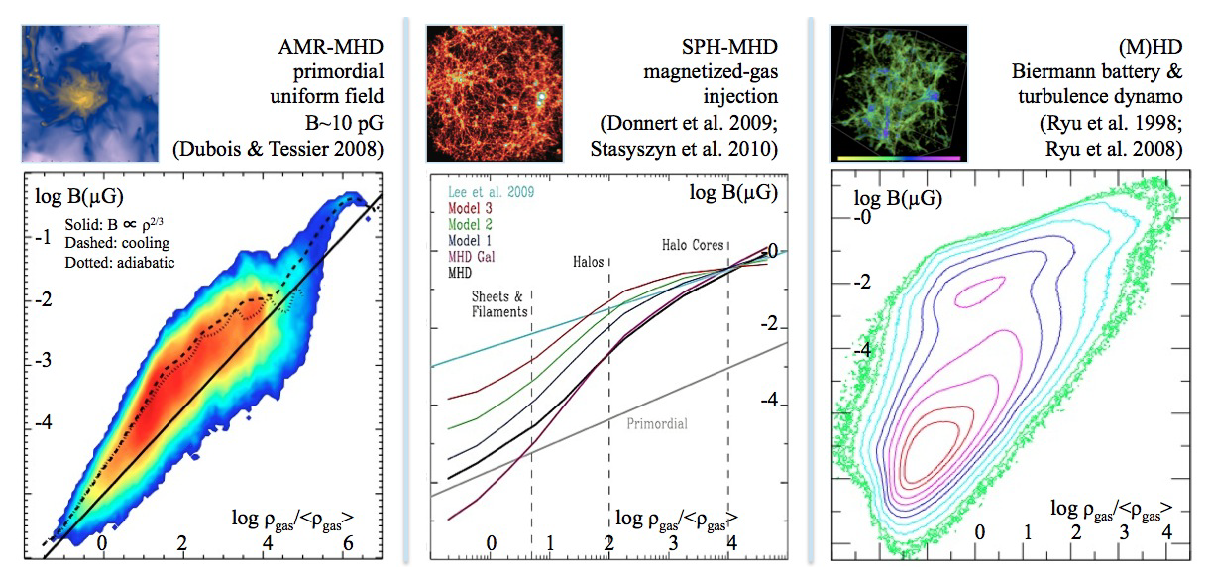
\includegraphics[width=0.8\linewidth]{magnetism/c06.s1.ss6.f1.eps}
\end{center}
\caption{
大規模構造の密度と磁場強度の宇宙論的シミュレーション。左から宇宙初期の一様な磁場からの進化モデル\citep{2008A&A...482L..13D}、AGNフィードバックで磁場を供給するモデル\citep{2010MNRAS.408..684S}、ビエマン効果による生成と乱流ダイナモによる成長のモデル\citep{2008Sci...320..909R}。
}\label{c06.s1.ss6.f1}
\begin{center}
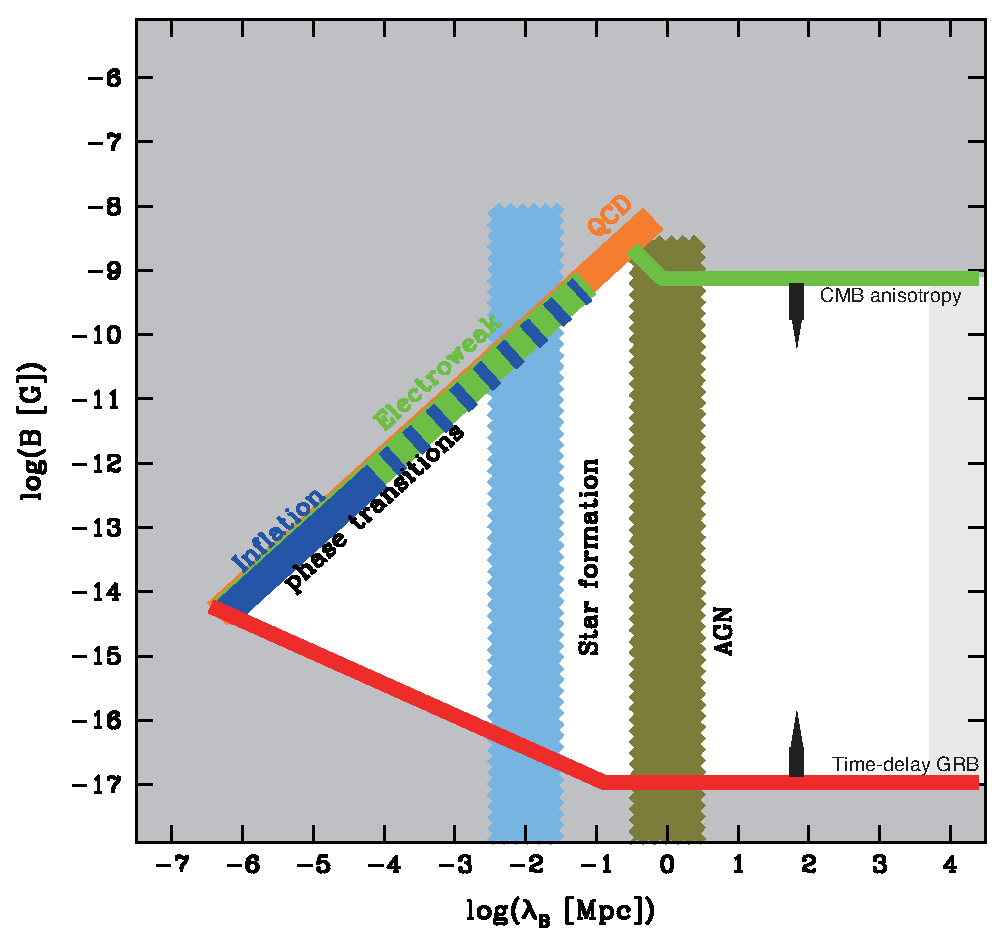
\includegraphics[width=0.7\linewidth]{magnetism/c06.s1.ss7.f1.eps}
\end{center}
\caption{宇宙論的磁場に対する観測と理論からの制限のまとめ。観測的な上限はCMBの温度揺らぎから、下限は2次的$\gamma$線が観測されていないことから得られている(本文参照)。図上で左下から右上へ伸びている制限は乱流による磁場のカスケードでのスケールの上限をあらわしている。\cite{2013A&ARv..21...62D}より改変。
}\label{c06.s1.ss7.f1}
\end{figure}

%%%%%%%%%%%%%%%%%%%%%%%%%%%%%%%%%%%%%%%%%%%%%%%
%%%%%%%%%%%%%%%%%%%%%%%%%%%%%%%%%%%%%%%%%%%%%%%
\subsection{宇宙論的磁場の科学的課題}
\label{c06.s1.ss7}

%%%%%%%%%%%%%%%%%%%%%%%%%%%%%%%%%%%%%%%%%%%%%%%
\subsubsection{はじめに}
\label{c06.s1.ss7.sss1}

\paragraph{宇宙最初の磁場:初期宇宙起源}

銀河や銀河団には銀河の大きさを超える相関長をもった(整列した)マイクロガウス程度の磁場が存在しているが、その起源は未だ解明されていない。例えば渦巻き銀河に限れば、銀河形成時に$10^{-20}$ G から $10^{-30}$ G程度の磁場が$\lambda_B\gtrsim 1$kpcの相関長をもって必要だといわれている\citep{1999PhRvD..60b1301D}。そういった相関長の長い磁場を含む、宇宙の磁場の起源の一つの候補として、初期宇宙に生成されたとする初期宇宙起源シナリオがある。

%%%%%%%%%%%%%%%%%%%%%%%%%%%%%%%%%%%%%%%%%%%%%%%
\subsubsection{宇宙論的磁場の理論}
\label{c06.s1.ss7.sss2}

\paragraph{インフレーション起源}

インフレーション期に長い相関長をもって生成された種磁場が、構造形成とともに増幅し現在のような磁場になったとする考え方がある。ここで、電磁場の理論は共形変換に対して不変であるため、電磁場の量子ゆらぎが生成されないという基本性質がある。そのため標準模型を超えた理論・アイデアが古くから様々に提案されてきた。例えば、ディラトン\citep{1992ApJ...391L...1R,2004PhRvD..69d3507B}、ヒッグス\citep{2004PhRvD..70d3004P}のようなスカラー場との結合や、重力との結合\citep{1988PhRvD..37.2743T}などである。インフレーション期による宇宙論的磁場生成の利点は、その加速的宇宙膨張によって磁場の相関長が十分長くとれることである。

\paragraph{インフレーション起源の問題}

最近、特に日本人研究者による大きな貢献により、インフレーション期に磁場を作るためには次のような矛盾点を解決しなくてはならないことが分かってきた:(i) 電磁場との相互作用が初期宇宙で強結合となってしまい、理論が摂動論的に扱えなくなってしまう\citep{2009JCAP...08..025D} (ii) 磁場を生成しようとすると、電場の方が大きくなってしまい、その反作用のためインフレーションが続かない\citep{2009JCAP...12..009K} (iii) 電磁場起源の密度揺らぎを作りすぎる\citep{2012PhRvD..86b3512S,2014JCAP...03..013F}。これらを総合すると、磁場は大きなスケール側で抑制されていることが必要となり、最も単純な$f^2(\phi)F_{\mu\nu}F^{\mu\nu}$型のモデルでは、Mpcの相関長で$B\lesssim10^{-30}$Gと制限されてしまう\citep{2014JCAP...06..053F}。 したがって、理論的な立場からはインフレーション期による磁場生成は難しい状況であるが、このことを観測的な立場から検証していくことは重要である。

\paragraph{インフレーション以外の磁場生成起源}

インフレーション期以外の磁場生成シナリオとしては、例えば宇宙再加熱期での磁場生成\citep{2014JCAP...05..040K}や、宇宙の相転移での磁場生成\citep{1983PhRvL..51.1488H,1991PhLB..265..258V}などがあり、これらの生成モデルに対しては上述のような制限はない。また、\cite{2013PhRvD..87h3007K}では、量子色力学(QCD)の相転移で生成された磁場は$50$kpcの相関長で$10^{-9}$G, 量子電磁力学(QED)の相転移では$0.3$kpcの相関長で$10^{-10}$G程度の強度が期待できると議論されている。インフレーション期以外の磁場生成では、宇宙の地平線を越えて磁場を増幅することができないため、小スケール側でエネルギーが卓越するという著しい特徴が挙げられる。

\paragraph{再結合時の磁場生成}

他にも相関長が長い種磁場を生成する物理過程として、再結合時でのベクトル型の揺らぎによる生成がある\citep{2005PhRvL..95l1301T}。特に密度揺らぎの摂動2次の効果によるものは、その揺らぎの統計的性質が観測より既知であるので、生成される磁場の強度、スペクトルも曖昧さなく求めることができる。1次の揺らぎの積による効果は既に\cite{2006Sci...311..827I}で求められ、純粋な摂動2次の効果を取り込んだ計算が\cite{1405.4810}で行われている。

\paragraph{今後の理論的課題}

上に述べたようにインフレーションでは大スケールの磁場生成が難しいことが明らかになりつつある一方で、インフレーション後、ビッグバンが始まる間での磁場生成であれば可能性がある\citep{2014JCAP...05..040K}。 また、他の可能性として、インフレーション時に小スケールでヘリシティを持った磁場を生成するモデルを構築することができれば、逆カスケードによって種磁場として十分な大きさの磁場を大スケールへ輸送することができるかもしれない。いずれにせよ、宇宙で天体形成が始まるまでの初期状態において、理論的に存在が許される磁場の強度、スペクトルを明らかにすることが理論での課題といえる。

%%%%%%%%%%%%%%%%%%%%%%%%%%%%%%%%%%%%%%%%%%%%%%%
\subsubsection{宇宙論的磁場の観測}
\label{c06.s1.ss7.sss3}

\paragraph{これまでの観測}

これまでの観測状況は宇宙大規模構造磁場の観測と共通する。とりわけボイド領域の銀河間磁場は構造形成の影響を受けていない可能性があり、宇宙初期の情報を残す宇宙論の貴重な探針となりうる。

\paragraph{課題}

宇宙論的磁場に対する観測的な制限はいくつかあるが、現時点でもっとも強い制限を与えているものは宇宙マイクロ波背景輻射温度揺らぎ(CMB)によるものと、$TeV$を越えるエネルギーをもつ$\gamma$線を放射する天体からの2次的$\gamma$線(TeV$\gamma$線が赤外線と反応して電子陽電子対を生成し、これら荷電粒子がCMB光子を逆コンプトン散乱して生成する)の遅延放射によるものである。前者は磁場が生成するCMB揺らぎが観測されている温度揺らぎを越えないことから$B\lesssim 3.4\times 10^{-9}$ Gという磁場に対するおよその上限がPlanck衛星により\citep{2012PhR...517..141Y,2013arXiv1303.5076P}、また後者はblazarからの$\gamma$線のカスケード放射がGeV領域で観測されていないことから$B\gtrsim 10^{-16}$ Gという磁場に対する下限が得られている\citep{2012ApJ...744L...7T,2010Sci...328...73N,2011A&A...529A.144T}。この$\gamma$線を用いた方法はジャイロ半径とinverse Compton 冷却距離の比較から得られる原理的な上限があり、$E_e$を$\gamma$線のエネルギーとして
\begin{equation}
B_{\rm max}\approx 3\times 10^{-15}~{\rm G}~\left(\frac{E_e}{1{\rm TeV}}\right)^2
\end{equation}
で与えられる\citep{2013A&ARv..21...62D}。これより強い磁場については高エネルギー宇宙線を用いる方法がある\citep{1995ApJ...455L..21L}。これらをまとめた図を図\ref{c06.s1.ss7.f1}に示す。観測的にはこの図の空白部分を埋めていくことが課題として挙げられる。


%%%%%%%%%%%%%%%%%%%%%%%%%%%%%%%%%%%%%%%%%%%%%%%
%%%%%%%%%%%%%%%%%%%%%%%%%%%%%%%%%%%%%%%%%%%%%%%
\subsection{ファラデートモグラフィーの科学的課題}
\label{c06.s1.ss8}

%%%%%%%%%%%%%%%%%%%%%%%%%%%%%%%%%%%%%%%%%%%%%%%
\subsubsection{はじめに}
\label{c06.s1.ss8.sss1}

\paragraph{ファラデートモグラフィーで何がわかるか?}

偏波強度スペクトル$P(\lambda^2)$はファラデースペクトル$F(\phi)$を用いて表すことができる(\S \ref{c06.s1.ss1.sss4})。ファラデースペクトルはファラデー深度$\phi$における偏波強度であり、ファラデー深度は熱的電子密度や視線方向に沿った磁場の強さによって表された。また偏波放射は主にシンクロトロン放射によるものでその強度は宇宙線電子と視線方向に垂直な磁場の強さで決まる。したがってファラデースペクトルは磁場、熱的電子(電離ガス)、宇宙線電子の視線方向分布によって決まることになる。逆に、観測されたファラデースペクトルからこれらの物理量に関する情報を得ることができる。偏波を放射している天体、もしくは放射していない領域をもトモグラフィーによって探索することができ、その応用範囲は銀河や銀河団、大規模構造、超新星残骸、活動銀河核など広範に及ぶと期待される。

\paragraph{銀河磁場研究への適用}

銀河をターゲットにした場合、2次元的なイメージングとファラデートモグラフィーを組み合わせることによって銀河の3次元構造を探ることができる。上述の物理量の分布には大局的な特徴と乱流による小スケールの特徴があり、銀河のダイナミクスに密接に関連している。特に銀河ダイナモや銀河磁場の起源の謎に迫ることができるだろう。銀河のファラデースペクトルの例を図\ref{c06.s1.ss8.f1}に挙げる\citep{2014PASJ...66....5I}。これは渦巻銀河の磁場、熱的電子、宇宙線電子の分布モデルに基づき、地球に円盤面を向けた(face-on)銀河の観測を想定した場合のファラデースペクトルである。まず左上図の視線方向磁場と電子密度から左下図のファラデー深度が計算され、これと偏波強度分布を合わせることによってファラデースペクトルが計算される。ファラデースペクトルの偏波角(右上)と偏波強度(右下)が$\phi$の関数として示されている。

\begin{figure}[tbp]
\begin{center}
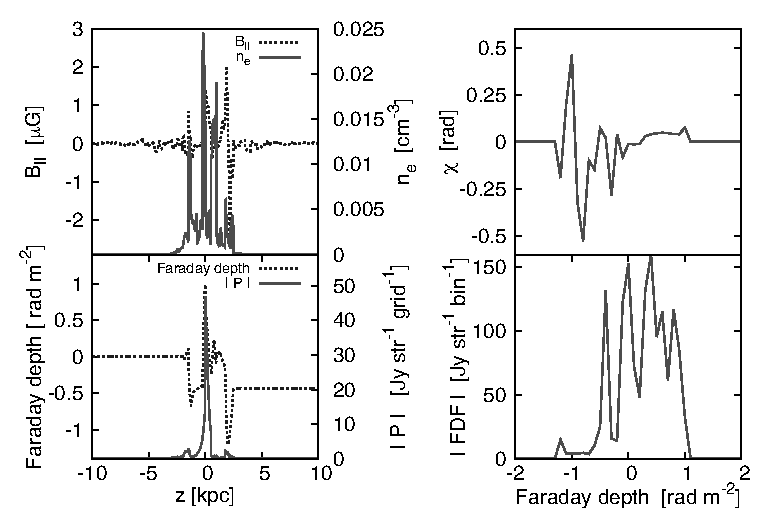
\includegraphics[width=0.7\linewidth]{magnetism/c06.s1.ss8.f1.eps}
%%%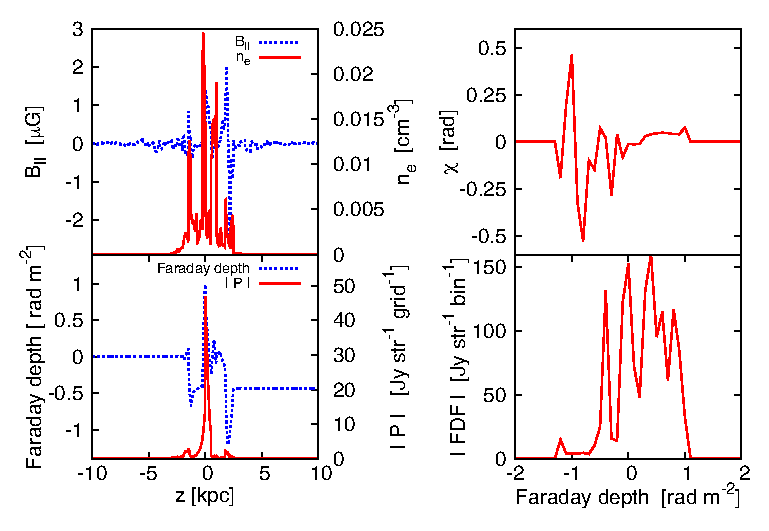
\includegraphics[width=0.7\linewidth]{magnetism/c06.s1.ss8.f1c.eps}
\end{center}
\caption{Face-onの渦巻銀河モデルより計算したファラデースペクトル\citep{2014PASJ...66....5I}。(左上)視線方向磁場と熱的電子の分布。(左下)偏波強度の分布と左上図に基づいて計算したファラデー深度。(右上)ファラデースペクトルの偏波角。(右下)ファラデースペクトルの絶対値。
}\label{c06.s1.ss8.f1}
\end{figure}

\paragraph{銀河間磁場研究への適用}

近傍の銀河を通して遠方の偏波源を観測してトモグラフィーを行なえば、2つの偏波源を$\phi$空間で分離して、実空間で2つの偏波源の間に存在する銀河間磁場をファラデースペクトルの中に同定できる可能性がある\citep{2014PASJ...66...65A}。従来の単純なファラデー回転を用いた方法では、磁場は偏波源から観測者まで積分したものしか得られないので、天体そのものや銀河系に付随する磁場を精度よく差し引くことが難しく、せいぜい$O(1)~{\rm rad~m^{-2}}$程度である銀河間磁場を検出することは非常に困難であったので、銀河間磁場の観測的研究はファラデートモグラフィによって大きく進展すると期待される。

\paragraph{2つの逆問題}

ファラデートモグラフィーによって銀河の3次元構造や銀河間磁場を探るにあたって2つの逆問題がある。1つは観測された偏波強度スペクトル$P(\lambda^2)$からどのようにファラデースペクトル$F(\phi)$を再現するか。もう1つは得られたファラデースペクトルの解釈、つまり$F(\phi)$からどのように物理的情報(磁場、熱的電子、宇宙線電子の分布)を引き出すかである。

%%%%%%%%%%%%%%%%%%%%%%%%%%%%%%%%%%%%%%%%%%%%%%%
\subsubsection{ファラデートモグラフィーの理論的課題1}
\label{c06.s1.ss8.sss2}

\paragraph{ファラデースペクトルの再構築}

$P(\lambda^2)$と$F(\phi)$は数学的にはフーリエ変換の関係にあるので、単純には逆変換をすることで$P(\lambda^2)$から$F(\phi)$を得ることができることはすでに紹介した。しかし、偏波強度$P(\lambda^2)$の定義域が$\lambda^2 > 0$であるため$\lambda \leq 0$の領域のデータは原理的に得ることができない。また$\lambda^2 > 0$の領域であっても望遠鏡の観測帯域によって限られてしまう。従って、逆フーリエ変換を完全に行うことはできず、不完全な観測データからできるだけ多くの情報を引き出すために様々な方法が考案されている。

\paragraph{逆変換法}

フーリエ逆変換によるノイズ混入と情報劣化を、様々な工夫によって改善する試みが行われている。例えばRM CLEAN法は、電波望遠鏡における像合成の1手法であるCLEANアルゴリズムと同様な方法で、ファラデースペクトルを再構築する\citep{2009IAUS..259..591H,2014PASJ...66...61K}。逆変換の質が良くないのは観測データが不完全であるためだが、圧縮サンプリング法では$F(\phi)$がスパース性というある種の単純さを持っていると仮定するとこれをよく再構築できる可能性がある\citep{2011A&A...531A.126L}。ウェーブレット変換法はそもそもフーリエ変換をやめるという試みである。ウェーブレット変換は、フーリエ変換が周期関数を基底とすることで生じる周期性の問題を克服するもので、ファラデートモグラフィーにも応用されている\citep{2010MNRAS.401L..24F}。

\paragraph{モデルフィット法}

$F(\phi)$の形を具体的に仮定し、観測された$P(\lambda^2)$にもっともよくフィットするように$F(\phi)$の形を特徴づけるパラメータを決める方法である。一般にデータ数に比べてパラメータ数が圧倒的に少ないため比較的質の悪いデータであってもパラメータはよく決まるが、あらかじめ$F(\phi)$の形を仮定しなければいけないところに問題点がある。

\paragraph{比較プロジェクト}

\cite{1409.4151}では$F(\phi)$を仮定してASKAPの観測シミュレーションを行い、様々な方法で$F(\phi)$の再現性を比較した。その結果は圧倒的にモデルフィット法の優位を示すものであったが、これは仮定した$F(\phi)$がデルタ関数やトップハット型関数などごく単純なものであったことに起因していると考えられる。現実の銀河のファラデースペクトルは複雑な形であり、どのような形の関数が現実の天体をフィットするのに適しているのかを考慮する必要がある。

\begin{figure}[tbp]
\begin{center}
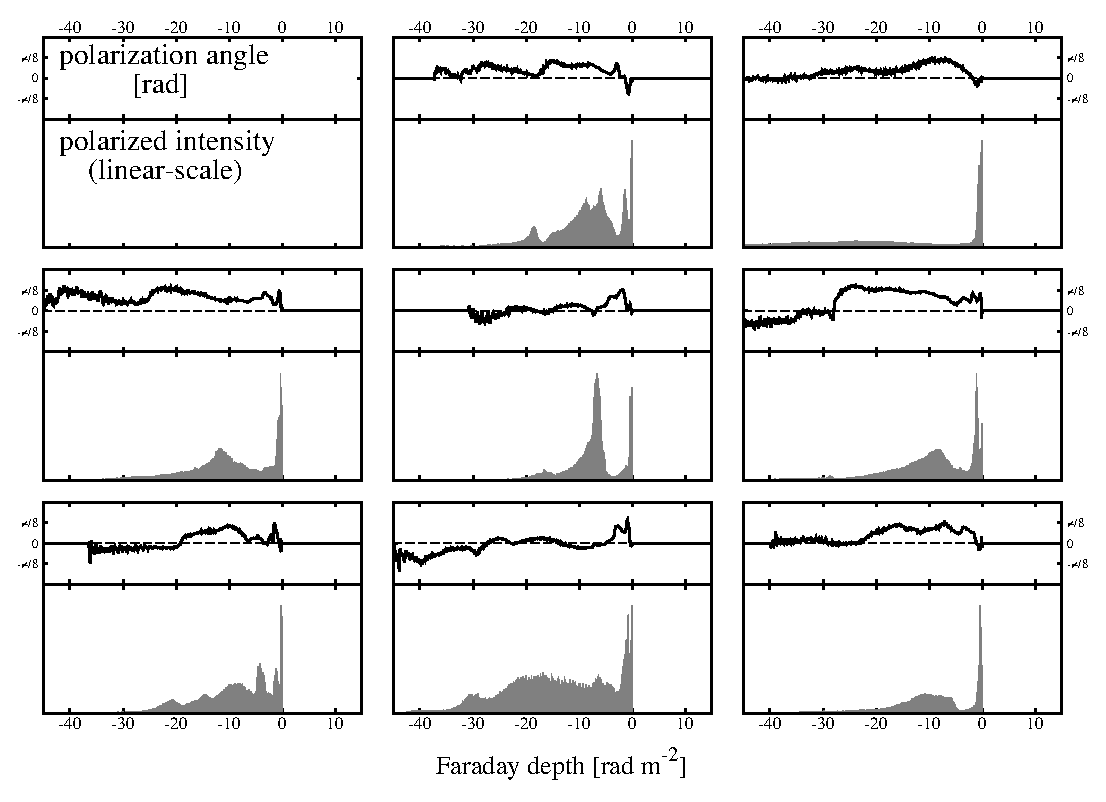
\includegraphics[width=0.7\linewidth]{magnetism/c06.s1.ss8.f2.eps}
\end{center}
\caption{face-onの渦巻銀河モデルより計算したファラデースペクトル\citep{2014PASJ...66....5I}。上段は偏波角、下段は偏波強度である。垂直磁場の強さや熱的電子・宇宙線分布のscale heightなど銀河の大局的なパラメータが同じでも、乱流の再現が異なるだけで形状はかなり異なるのが分かる。
}\label{c06.s1.ss8.f2}
\end{figure}

%%%%%%%%%%%%%%%%%%%%%%%%%%%%%%%%%%%%%%%%%%%%%%%
\subsubsection{ファラデートモグラフィーの理論的課題2}
\label{c06.s1.ss8.sss3}

\paragraph{ファラデースペクトルの解釈}

ファラデースペクトルを観測データから再構築することができたとして、例えば銀河について我々が知りたい情報は、大局的な磁場の形状と強さ、熱的電子や宇宙線の密度分布、乱流の特徴的なスケール・強さや空間スペクトルだろう。ところが、一般にファラデースペクトルからこれらの物理的な情報をどう引き出せるかは自明ではなく、そして単純ではない。図\ref{c06.s1.ss8.f2}にはいくつかの銀河モデルに対するファラデースペクトルの偏波角と偏波強度が$\phi$の関数としてプロットされているが、その形状は非常に複雑であることがわかる。実はこれらのファラデースペクトルは全て同じ銀河モデル、つまり垂直磁場の強さや熱的電子・宇宙線分布のscale heightなど銀河の大局的なパラメータが等しい銀河モデルのもので、ただ乱流の再現だけが異なるのである。それにも関わらず、ピークの数や幅などに関して驚くほど多様である。これをどう特徴付けし物理的に解釈するかは今後の課題で、\cite{2014PASJ...66....5I}ではファラデースペクトルの形をその広がりや歪度、尖度などで特徴づけて物理的情報を引き出す試みをしているが、今後さらなる研究が必要である。



